\chapter{Background}

\section{Motivation}
As life expectancy increases in Norway, so does the population who needs geriatric care either at home, or in a geriatric facility. From \cite{webstat:oslo:hjsyk} we can see that both the number of people in need home nursing is steadily increasing across all amounts of assistance needed. In addtion, the time spent per user has also increased over the years. This means that the time geriatric personnel has, must be spent more efficiently, and with the users that need the most help. We propose a novel robotic system that can monitor an elderly person (from here on called ``the user'') living at home and give feedback to healtcare personnel about their health, and how much assistance is needed. The system should also be able to detect and predict abnormal states of the user, and warn the appropriate emergency services.

This work will focus on creating data that can be used to model the current state of the subject, as well as implementing models predicting future states. In this effort we wish to monitor the subject's medical data such as respiration rate (RR) and heart rate (HR), daily activities and mood, as well as  contextual input such as the ambient temperature, weather, nearby objects and current location. Machine learning models focusing on both short and long term prediction is discussed. 



%% Asymmetry in gait after stroke. -> detect and report?



%% \section{Elderly Care}
\subsection{Facilities}
Elderly people are often put in homes to better get help with their needs.
\subsection{Living at Home}
Home nursery

%% \section{Multimodal Elderly Care System}
A system to assist elderly living at home. 



%% As we are ever growing older, and staying at home until a greater age, we need to help healthcare personell to provide their services to the people that need it the most. This will help them spend their limited time more efficiently, and possibly provide 

%% This project describes a system for obtaining vital data from a subject for the purposes of modelling the subjects state. It also implements methods for predicting future states based on predetermined risk factors, contextual input, and the observed subject's historical data.


%% Contextual information: The users contemporary environment represents situational hazards and could provoke, or lessen the possibility of, certain events. For example, a day with high temprature and humidity coupled with activity could provoke dehydration and cause a fall. If such conditions are correctly assessed, preventative measures could be taken, such as suggesting to lower the temprature, take refuge in the shade, or asking to provide a glass of water.


%% \subsection{RGBD Sensor}
%% Widley used already implemented robotic systems. Using this sensor will give us a plethora of different alternative robotic platforms to base the system on. There are also many preexisting datasets for activity recognition using RGBD sensor to train the system on. An RGBD sensor has also been used to extract vital information from the video stream.
%% The RGBD sensor is also especially developed for estimating human pose, which can help in recognizing human positure and as mentioned activity.
%% In addition the sensor is versatile, and can be used for mapping and navigation as well.

%% \subsection{Jetson TX2}
%% In our experiments the Jetson TX2 board was used to preform human detection in the RGBD image using the OpenPose software developed by the CMU Perceptual Computing Lab. 

%% Pose detection 2d pose detection was done with the help of the OpenPose pretrained network. We then extract the 3d keypoints by projecting and scaling a rigid skeleton onto the depth image. Unobserved points are estimated using previous data, or confined to obstructed space and the kinematics of the skeleton.

%% Tracking the tracking of each person in the scene is done using face recognition and a simple kalman filter to predict the next location of each person. The faces are pre-stored on the system, and only anonymized information is sent over the network.

%% The software also supports tracking using multiple RGBD cameras, and will yield a more precise result. 

%% RoI extraction is done simply by making a box that contains all detected keypoints. We do the same for respective face and chest RoIs.

%% Mood extraction using the Face RoI detected, we run a mood recognition algorithm on the subject. This is done on system to prevent personal information being sent over the network.

%% Vitals are extracted using spacio temproal methods described in MiT methods, and built upon by various others.

%% Human Activity Recognition was traind on various RGBD datasets.

%% Propose decision tree or unsupervised learning model to detect anomalies in the daily routines.

%% Bottom Up
%% We then want to be able to predict what the person will experience in the near future, AND be able to take preventative measurements so that doesn't happen.
%% We could imagine a decision tree, and then suggest the available descisions that does not lead to the event we're trying to avoid -- kind of like a chess bot that would always choose the maximum possibility route for winning. However the problem is creating the decision tree. We need data, and know at exactly which moment a decision is being made.
%% We could look at the life of the subject as a series of predetermined, reliably recognizable actions. Then, we think of the actions as edges, or decisions, that lead to new states. In each state, we would also have a set of parameters describing the persons vitals and environmental conditions. If all actions are possible in any state, we need to record the similarities beteween different peoples strings of actions. We want the likeleyhood of a person taking a certain action given a set of parameters, and wether or not that action led to a fall or another undesirable event or not.

%% For this a Hidden Marov Model could be used. The problem is obtaining the training data.
%% We could make the training data synthetically to train the model, and then retrain it using actual data when the system is live. However, this might be immoral, in that we would have to actually get the system to fail to learn anything. If the system never fails, we could be stuck in a local optimum where unneccessarily many restrictions are suggested to the subject.

\section{Remote Vital Monitoring}

Vital data such as respiration rate (RR) and heart rate (HR) could be useful to detect whether a person is undergoing stress, is relaxed, or help paint a more complete picture of the subject's current state. The temporal development of the vitals could also be valuable information to first responders in the event of an accident.
In this project we will rely on eulerian video magnification~\cite{Wu12Eulerian} to extract this data. The color channel of a camera will be used to detect changes in the color of the skin at different keypoints on the face of a person to detect the HR.
We also propose to use the depth channel of an RGB-D sensor to detect the rise and fall of a persons chest to estimate the RR.

\section{Human Pose Estimation}

Single view

A lot of work has already been done in detecting human pose, however our system has to work in real life environments where multiple different people can enter the scene. The system also needs to be able to run in real-time if rapid developments are happening. Therefore we will rely on the OpenPose~\cite{cao2017realtime} for initial 2D detection of people in the scene. However, to make the system robust to changes in perspective, so we wish to extract the 3D pose of each person using the depth information from an RGB-D sensor.
A tracker should also be implemented to ensure object permanence and separate recorded data from multiple people.

\begin{figure}
  \begin{floatrow}
    \ffigbox{
      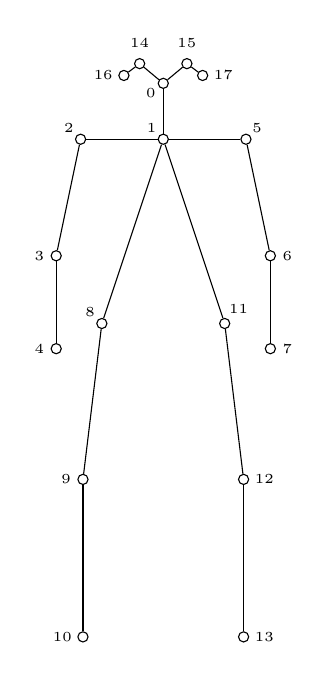
\begin{tikzpicture}[
          every node/.style={draw,circle,minimum size=.06cm, inner sep=1.3pt}
        ]
        \tiny
        %% \draw[help lines, step=5mm, gray!20] (-4,-4) grid (3,4);
        
        \node[label={[label distance=-.2mm]200:{0}}] (nose) at (0,3.25) {};
        \node[label={[label distance=-.2mm]140:{1}}] (neck) at (0,2.54) {};
        
        \node[label={[label distance=-.1mm]90:{14}}] (reye) at (-.3,3.5) {};
        \node[label={[label distance=-.1mm]90:{15}}] (leye) at (.3,3.5) {};

        \node[label={[label distance=-.1mm]180:{16}}] (rear) at (-.5,3.35) {};
        \node[label={[label distance=-.1mm]0:{17}}] (lear) at (.5,3.35) {};

        \node[label={[label distance=-.2mm]140:{2}}] (rshoulder) at (-1.05,2.54) {};
        \node[label={[label distance=-.2mm]50:{5}}] (lshoulder) at (1.05,2.54) {};
        
        \node[label={[label distance=-.1mm]180:{3}}] (relbow) at (-1.36,1.06) {};
        \node[label={[label distance=-.1mm]0:{6}}] (lelbow) at (1.36,1.06) {};

        \node[label={[label distance=-.1mm]180:{4}}] (rwrist) at (-1.36,-.12) {};
        \node[label={[label distance=-.1mm]0:{7}}] (lwrist) at (1.36,-.12) {};

        \node[label={[label distance=-.2mm]140:{8}}] (rhip) at (-.78,.2) {};
        \node[label={[label distance=-.2mm]50:{11}}] (lhip) at (.78,.2) {};

        \node[label={[label distance=-.1mm]180:{9}}] (rknee) at (-1.02,-1.78) {};
        \node[label={[label distance=-.1mm]0:{12}}] (lknee) at (1.02,-1.78) {};

        \node[label={[label distance=-.1mm]180:{10}}] (rankle) at (-1.02,-3.78) {};
        \node[label={[label distance=-.1mm]0:{13}}] (lankle) at (1.02,-3.78) {};

        %% \draw[blue] (0,0) circle [radius=.06cm];

        \draw (nose) -- (neck);
        \draw (reye) -- (nose); \draw (leye) -- (nose);
        \draw (reye) -- (rear); \draw (leye) -- (lear);
        
        \draw (neck) -- (rshoulder); \draw (neck) -- (lshoulder);
        \draw (neck) -- (rhip); \draw (neck) -- (lhip);

        \draw (rshoulder) -- (relbow); \draw (lshoulder) -- (lelbow);
        \draw (rwrist) -- (relbow); \draw (lwrist) -- (lelbow);

        \draw (rhip) -- (rknee); \draw (lhip) -- (lknee);
        \draw (rknee) -- (rankle); \draw (lknee) -- (lankle);
      \end{tikzpicture}
    }
    {
      \label{fig:openpose_skeleton}
      \caption[Numbering for OpenPose's keypoint markers]{Numbering for OpenPose's keypoint markers.}
    }
    %% \end{figure}
    %% \begin{table}
    \capbtabbox{
      \begin{tabular}[H]{|r l|}
        \hline
        ID & Name \\ \hline
        0  & Nose \\
        1  & Neck \\
        2  & Right Shoulder \\
        3  & Right Elbow \\
        4  & Right Wrist \\
        5  & Left Shoulder \\
        6  & Left Elbow \\
        7  & Left Wrist \\
        8  & Right Hip \\
        9  & Right Knee \\
        10 & Right Ankle \\
        11 & Left Hip \\
        12 & Left Knee \\
        13 & Left Ankle \\
        14 & Right Eye \\
        15 & Left Eye \\
        16 & Right Ear \\
        17 & Left Ear \\
        \hline
      \end{tabular}
    }{
      \label{tab:openpose_body_ids}
      \caption[IDs for OpenPose keypoint markers]{IDs for OpenPose's keypoint markers.}
    }
  \end{floatrow}
\end{figure}


\section{Human Activity Recognition}

In this part of the project we will compare Hidden Markov Models to Long Short Term Memory (LSTM) networks to recognize and predict different human activities using datasets such as~\cite{sung_rgbdactivity_2012},~\cite{h36m_pami} and~\cite{berkeley_mhad}.

\subsection{Human habits}
We compare Hidden Markov Models to LSTM networks in an effort to detect abnormal patterns in the subject's daily/weekly routines.

\section{Technologies}
\subsection{Robotic Operating System}
The Robotic Operating System (ROS) is a open source framework for building robotic applications used by both academia and in an increasing degree by robots in the industry. ROS provides us with a wide variety of tools and libraries developed by specialized laboratories from around the world. These tools and libraries makes it easier to communicate with different sensors, ready libraries for computer vision and spacial transformations, visualize motion, simulate input and get an overview of the general architecture of the system.
In this project we will for example use the iai\_kinect2 package~\cite{iai_kinect2} as well as the OpenCV library~\cite{opencv_library}.

One of the most useful parts of ROS is that we can easily connect different programs together using ROS messages, topics and pipelines. We can therefore tie together the different parts of this system without much effort, and is why it was chosen as the framework for this project.

%% \subsection{Open Pose}


\subsection{Red Green Blue Depth (RGB-D)}
An RGDB-D sensor was chosen for this project, as this kind of sensor is already widely used in robotic applications. This makes the package more portable, and can suit many different robot configurations. Using RGB-D data, we also get access to preexisting datasest for training our system. The Microsoft Kinect sensor was used in testing and development.

\subsubsection{Stereo vision}

\subsubsection{Scattered light}

\subsubsection{Long Short Term Memory}



\subsection{}
%% \subsubsection{Depth perception}

%% \subsubsection{Structured Light}

